\documentclass[acmlarge]{acmart}

\usepackage{booktabs} % For formal tables
\usepackage{xxxnotes} 
\usepackage{tikz}
% Metadata Information
%\acmJournal{PACMHCI}
%\acmVolume{9}
%\acmNumber{4}
%\acmArticle{39}
%\acmYear{2010}
%\acmMonth{3}
%\acmArticleSeq{11}

%\acmBadgeR[http://ctuning.org/ae/ppopp2016.html]{ae-logo}
%\acmBadgeL[http://ctuning.org/ae/ppopp2016.html]{ae-logo}


% Copyright
%\setcopyright{acmcopyright}
%\setcopyright{acmlicensed}
%\setcopyright{rightsretained}
%\setcopyright{usgov}
%\setcopyright{usgovmixed}
%\setcopyright{cagov}
%\setcopyright{cagovmixed}

% DOI
%\acmDOI{0000001.0000001}

% Paper history
%\received{February 2007}
%\received{March 2009}
%\received[accepted]{June 2009}


% Document starts
\begin{document}
% Title portion
\title{The Price of Human Behaviors}

\author{Lillian Tsai}
\orcid{1234-5678-9012-3456}
\affiliation{%
  \institution{MIT}
  \city{Cambridge}
  \state{MA}
  \country{USA}}
\email{tslilyai@mit.edu}
\author{Vibhaalakshmi Sivaraman}
\affiliation{%
  \institution{MIT}
  \city{Cambridge}
  \state{MA}
  \country{USA}}
\email{vibhaa@mit.edu}
\author{Xiaoyue Gong}
\affiliation{%
  \institution{MIT}
  \city{Cambridge}
  \state{MA}
  \country{USA}}
\email{xygong@mit.edu}

\begin{abstract}
The impact of selfish actions on the latency incurred by a network users has historically been a problem of great interest to the algorithmic community. Our paper first presents a brief overview of the original selfish routing problem, the standard algorithms used to route in the selfish routing setting, and the limits on the optimality of these algorithms (termed as the ``price of anarchy"), and then compare and contrasts other recent works that have formulated the problem in
    (perhaps more realistic) settings, i.e., by taking into account the possibility for altruistic, risk averse, and diverse-interest behaviors.  This paper both presents and clarifies the findings of these papers in the context of the original selfish routing paper, and demonstrates how these papers' results can be synthesized into a more general framework addressing optimality of routing with various human behaviors or motivations.
\end{abstract}

\keywords{selfish routing, price of anarchy}

\maketitle

%%%%%%%%%%%%%%%%%%%%%%%%%%%%%%%%%%%%%%%%%%%%%%%%%%%%%%%%%%%%%%%%%%%%%%%%%%%%%%%%%%%%%%%%%%%%%%%%
%%%%%%%%%%%%%%%%%%%%%%%%%%%%%%%%%%%%%%%%%%%%%%%%%%%%%%%%%%%%%%%%%%%%%%%%%%%%%%%%%%%%%%%%%%%%%%%%
%%%%%%%%%%%%%%%%%%%%%%%%%%%%%%%%%%%%%%%%%%%%%%%%%%%%%%%%%%%%%%%%%%%%%%%%%%%%%%%%%%%%%%%%%%%%%%%%
\section{Introduction}
Finding the best strategy for network and traffic routing has historically been a problem of great importance combining the theoretical aspects of both game theory and computer science. 
\begin{itemize}
    \item Introduce noncooperative games / Nash equilibrium (in network setting)
    \item Briefly introduce selfish routing paper / price of anarchy
    \item Discuss how it is a limited view of human behavior
    \item Briefly discuss alternatives (papers including taxes, etc.)
    \item There are newer papers with more interesting versions of human behavior
    \item We present a survey of these newer papers to show how human behaviors affect price of anarchy
\end{itemize}

%%%%%%%%%%%%%%%%%%%%%%%%%%%%%%%%%%%%%%%%%%%%%%%%%%%%%%%%%%%%%%%%%%%%%%%%%%%%%%%%%%%%%%%%%%%%%%%%
%%%%%%%%%%%%%%%%%%%%%%%%%%%%%%%%%%%%%%%%%%%%%%%%%%%%%%%%%%%%%%%%%%%%%%%%%%%%%%%%%%%%%%%%%%%%%%%%
%%%%%%%%%%%%%%%%%%%%%%%%%%%%%%%%%%%%%%%%%%%%%%%%%%%%%%%%%%%%%%%%%%%%%%%%%%%%%%%%%%%%%%%%%%%%%%%%
\section{Background}
This section presents a brief history of traffic routing algorithms, defining the terminology
and the traffic routing problem.

\subsection{The Traffic Routing Problem}
Traffic routing problems naturally arise in communication or transportation networks, where
links in the network often becomes \emph{congested} if too many users decide to route their data 
or cars through that link. In these networks, the path each user chooses can affect the travel times of other
users. Here, we describe Roughgarden and Tardos' formalization of the problem as multicommodity flow networks~\cite{tardos,roughgarden}, and use Pigou's example network in Figure~\ref{fig:Pigou} as a running example.

\begin{figure}[ht!]
\begin{center}
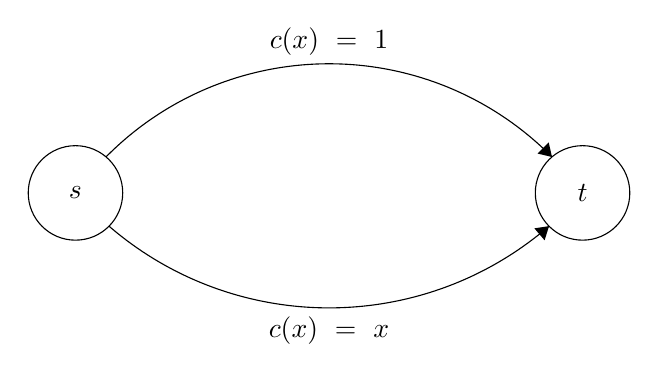
\begin{tikzpicture}[scale=0.2]
\tikzstyle{every node}+=[inner sep=0pt]
\draw [black] (18,-17.9) circle (3);
\draw (18,-17.9) node {$s$};
\draw [black] (50.2,-17.9) circle (3);
\draw (50.2,-17.9) node {$t$};
\draw [black] (19.94,-15.615) arc (135.3471:44.6529:19.905);
\fill [black] (48.26,-15.62) -- (48.05,-14.69) -- (47.34,-15.4);
\draw (34.1,-9.2) node [above] {$c(x)\mbox{ }=\mbox{ }1$};
\draw [black] (48.072,-20.011) arc (-49.23907:-130.76093:21.4);
\fill [black] (48.07,-20.01) -- (47.14,-20.15) -- (47.79,-20.91);
\draw (34.1,-25.7) node [below] {$c(x)\mbox{ }=\mbox{ }x$};
\end{tikzpicture}
\end{center}
    \caption{Pigou's example traffic routing problem, with a demand of $r_{(s,t)} = 1$}
\label{fig:Pigou}
\end{figure}

\medskip\noindent
\textbf{The input} to a traffic routing problem consists of:
\begin{itemize}
    \item A network $G = (V, E)$ of $|V|$ destinations (e.g., locations or servers) and $|E|$ links 
    \item A set of $k$ source-destination pairs $S=\{(s_1,t_1), \cdots (s_k,t_k)\}$ representing traffic demands
    \item A {rate} $r_i$ of traffic for each $(s_i,t_i)\in S$ representing the demanded amount of traffic from $s_i$ to $t_i$
    \item A {latency} cost function $c$ that assigns a per-edge function $c_e$ to each edge $e$ describing how adding traffic (i.e., congestion) to $e$ affects how long it takes to travel time across $e$. We can also think of $c$ as assigning per-path costs: for any path $p$ in the graph
        $$c_p(f) = \sum_{e\in P}c_e(f_e)$$ 
        We assume that $c$ is continuous, nonnegative, and nondecreasing.
\end{itemize}
In Figure~\ref{fig:Pigou}, we see a single source-destination input network with an example (linear) cost function with $r_{(s,t)} = 1$.

\medskip\noindent
\textbf{Solutions} correspond to flow assignments to the set of simple paths $P_i$ between $s_i$ and $t_i$ for all $i$.\footnote{Note that our solutions assume \emph{nonatomic} entities: the flows we find may not be integral. 
Intuitively, this means that the demand from one $s_i$ to $t_i$ is generated by an infinite number
of entities in the network, which allows us to reason about continuous, rather than discrete, functions.}
%
To describe a flow assignment $f$, we can consider $f_p$, the flow on a single path $p \in P_i$ (this adds an equal amount of flow $f_p$ to all edges in $p$), as well as $f_e = \sum_p \sum_{e\in p} f_p$, the edge flow on edge $e$ (the sum of flow on all paths that use $e$).

A \emph{feasible} solution given such an input is an assignment of path flows such that the demand from $s_i$ to $t_i$ is met:
$$\forall i,~\sum_{p\in P_i} f_p = r_i$$
%
An \emph{optimal} (feasible) solution given such an input is the feasible flow assignment $f$ that minimizes the \textbf{total weighted cost} $C(f)$, where
$$C(f) = \sum_i\sum_{p\in P_i}c_p(f)f_p = \sum_{e\in E} c_e(f_e)\cdot f_e$$
Intuitively, we are calculating the cost of each path of a given flow assignment, weighing 
each path's cost proportional to the amount of flow through the path. More concretely,
if we were to let flow represent the routes chosen by (infinitely many) users, $C(f)$ calculates the average cost over all users. Thus, when minimizing $C(f)$, some users may incur 
more latency so that other users can go faster.
Note that there exists an optimal flow $f^*$ minimizing $C(f)$ because we assume $c$ is continuous and the set of feasible flows is compact.

In our running example (Figure~\ref{fig:Pigou}), a feasible flow is any flow that sends one unit from $s$ to $t$ (divided in any fashion between the top and bottom edges).
The optimal flow is the flow that sends half the traffic through the lower edge and half through the upper edge: the users on the lower edge only experience a cost of $1/2$, while the users on the upper edge experience a cost of $1$, making the total weighted cost $3/4$.

\subsection{Coordination Models and the Price of Anarchy}
Before we can create algorithms to solve the traffic routing problem, we must first assume a \emph{coordination model} for our traffic network.
There are two clear extremes: (1) centralized control, in which some entity (e.g., an air traffic controller) knows all traffic demands and routes accordingly, and
(2) decentralization, i.e., a complete \emph{lack} of coordination between
entities in the network.
In a centralized setting, there is a clear optimal solution, as shown in the previous section.
However, in a decentralized and uncoordinated model, the lack of coordination can result in
inefficiencies. 

\medskip
\textbf{The Price of Anarchy} (PoA) allows us to measure the inefficiencies of a decentralized model given some notion of equilibrium (how the flow assignment is determined in the model), and was first introduced by Koutsoupias and Papadimitriou in 1999~\cite{poa}. 
The PoA is defined as the ratio between the optimal flow and the flow achieved
at equilibrium.
(This is similar to how we measured the distance from optimal of an approximation algorithm in a limited computational power model, and of online algorithms in an incomplete information model.)

\subsection{The Selfish Routing Model}
One example of an uncoordinated model is the \emph{selfish routing} model, in which all entities in the network are selfish and choose a route minimizing their individual latency without caring (or knowing) about the effects on other users~\cite{tardos}.

The selfish routing model corresponds to flows at a \emph{Wardrop, or Nash equilibrium}~\cite{wardrop,haurie}.
The set of flows in a Wardrop equilibrium are defined such that for all $i$ source-destination pairs, all the paths from $s_i \to t_i$ have the minimum-possible cost. In other words, the (nonzero) 
flow paths at Wardrop equilibrium have equal path costs: 
$$\forall i,~\forall p_1, p_2\in P_i,~f_{p_1} > 0 \implies c_{p_1}(f) = c_{p_2}(f)$$

If we revisit our running example in Figure~\ref{fig:Pigou}, we note that the flow at Wardrop equilibrium corresponds to a flow that sends the entire unit of traffic through the bottom edge (the 0 flow through the top path has a cost of 1, and the unit flow through the bottom path will have cost 1).
Intuitively, each user routing from $s$ to $t$ will selfishly choose to take the bottom route because she will reason that the bottom route can have cost no worse than the top route. However, by doing so, the bottom route becomes more congested and leads to a total average cost $C(f) = 1$.
Thus, in Figure~\ref{fig:Pigou}, the price of anarchy is $\frac{1}{3/4} = \frac{4}{3}$.

\XXX{TODO should put more results about flows at Wardrop equilibrium? Not sure if important}

We next describe and present the main results regarding the PoA in this (decentralized) selfish routing model, which will act as a basis to which we will compare traffic routing results in more recently formulated models.

\XXX{TODO put results here}

%%%%%%%%%%%%%%%%%%%%%%%%%%%%%%%%%%%%%%%%%%%%%%%%%%%%%%%%%%%%%%%%%%%%%%%%%%%%%%%%%%%%%%%%%%%%%%%%
%%%%%%%%%%%%%%%%%%%%%%%%%%%%%%%%%%%%%%%%%%%%%%%%%%%%%%%%%%%%%%%%%%%%%%%%%%%%%%%%%%%%%%%%%%%%%%%%
%%%%%%%%%%%%%%%%%%%%%%%%%%%%%%%%%%%%%%%%%%%%%%%%%%%%%%%%%%%%%%%%%%%%%%%%%%%%%%%%%%%%%%%%%%%%%%%%
\section{Alternative Models}

\subsection{Altruistic}
\subsubsection{Model}
\subsubsection{Results}

%%%%%%%%%%%%%%%%%%%%%%%%%%%%%%%%%%%%%%%%%%%%%%%%%%%%%%%%%%%%%%%%%%%%%%%%%%%%%%%%%%%%%%%%%%%%%%%%
%%%%%%%%%%%%%%%%%%%%%%%%%%%%%%%%%%%%%%%%%%%%%%%%%%%%%%%%%%%%%%%%%%%%%%%%%%%%%%%%%%%%%%%%%%%%%%%%
%%%%%%%%%%%%%%%%%%%%%%%%%%%%%%%%%%%%%%%%%%%%%%%%%%%%%%%%%%%%%%%%%%%%%%%%%%%%%%%%%%%%%%%%%%%%%%%%
\subsection{Risk Adverse}
\subsubsection{Model}
\subsubsection{Results}

%%%%%%%%%%%%%%%%%%%%%%%%%%%%%%%%%%%%%%%%%%%%%%%%%%%%%%%%%%%%%%%%%%%%%%%%%%%%%%%%%%%%%%%%%%%%%%%%
%%%%%%%%%%%%%%%%%%%%%%%%%%%%%%%%%%%%%%%%%%%%%%%%%%%%%%%%%%%%%%%%%%%%%%%%%%%%%%%%%%%%%%%%%%%%%%%%
%%%%%%%%%%%%%%%%%%%%%%%%%%%%%%%%%%%%%%%%%%%%%%%%%%%%%%%%%%%%%%%%%%%%%%%%%%%%%%%%%%%%%%%%%%%%%%%%
\subsection{Diverse in Interests}
\subsubsection{Model}
\subsubsection{Results}


%%%%%%%%%%%%%%%%%%%%%%%%%%%%%%%%%%%%%%%%%%%%%%%%%%%%%%%%%%%%%%%%%%%%%%%%%%%%%%%%%%%%%%%%%%%%%%%%
%%%%%%%%%%%%%%%%%%%%%%%%%%%%%%%%%%%%%%%%%%%%%%%%%%%%%%%%%%%%%%%%%%%%%%%%%%%%%%%%%%%%%%%%%%%%%%%%
%%%%%%%%%%%%%%%%%%%%%%%%%%%%%%%%%%%%%%%%%%%%%%%%%%%%%%%%%%%%%%%%%%%%%%%%%%%%%%%%%%%%%%%%%%%%%%%%
\section{Discussion}
\subsection{Importance of Human Understanding}
\subsection{Future Work}
Clearly the models we present are a miniscule subset of all potential models for human behavior; 
furthermore, they are coarse-grained and oversimplistic in comparison with the complexity of the human
brain. As understanding of the neurophysiological aspects of human behavior improves, we hope to see a matching evolution in the precision and accuracy of these models for traffic routing as well.

\bibliography{paper}
\bibliographystyle{acm}

\end{document}
